\documentclass[onecolumn,aps, pre,amsmath,amssymb,longbibliography,11pt]{revtex4-2}
\usepackage{graphicx}
% \usepackage{dcolumn}
\usepackage{bm}
\usepackage{amsfonts}
\usepackage{xcolor,tabu}
\usepackage{multirow}
\usepackage{amsthm}
\usepackage{textcomp}
\usepackage{tikz}
\usepackage[colorlinks=true,
            linkcolor=blue,
            urlcolor=blue,
            citecolor=blue]{hyperref}
\hypersetup{bookmarksopen=true}
\usepackage{xr}
\usepackage{float}

\begin{document}
\title{Droplet tracking}
\maketitle

We study the motion of liquid droplets immersed in bacterial suspensions, an active bath.
The most basic and foundamental observation on the motion is the trajectory.
To obtain trajectories from a large amount of images, we need to develop an automatic tracking software.
Figure~\ref{fig:sample-image}A shows a sample image from an experiment, and the goal is to find the inner droplet, as highlighted in Fig.~\ref{fig:sample-image}B.

\begin{figure}[h]
  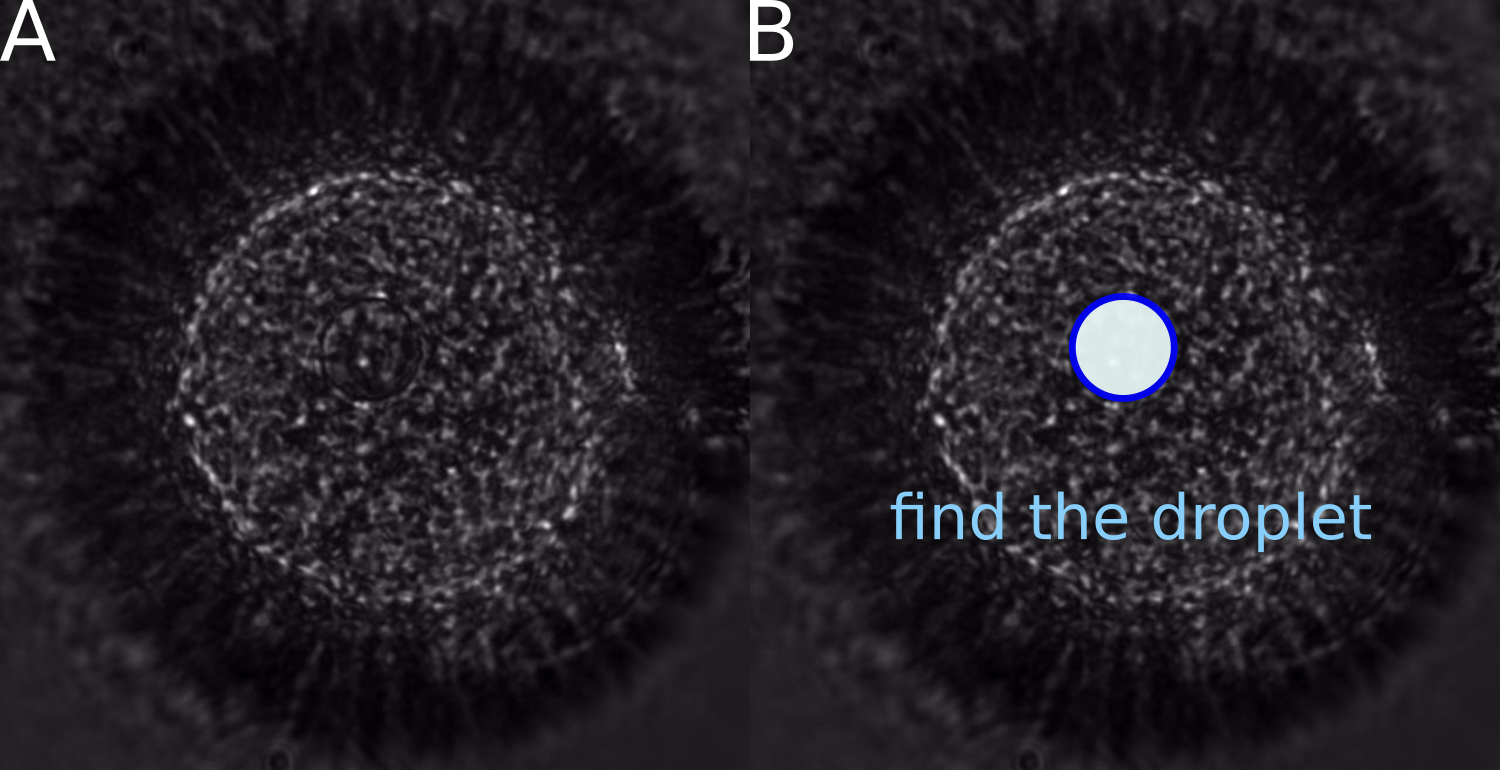
\includegraphics{sample-image.png}
  \caption{Sample image (A) and the goal of tracking software (B).}
  \label{fig:sample-image}
\end{figure}

\section{X-Y plane tracking}

\subsection{corrTrack}

I use corrTrack as the first attempt to find the inner droplet in the X-Y plane.
A description of corrTrack can be found in \href{https://github.com/ZLoverty/Python/tree/master/Tracking/corrTrack}{my Github repository}.
In this attempt, I used a binarized black circle as the mask (Fig.~\ref{fig:mask-and-result} inset), instead of a crop of the original image.
I did this because it is more general.
If the binarized mask works, it is very likely that a more specific mask, such as one cropped from the original image, will work.

\begin{figure}[h]
  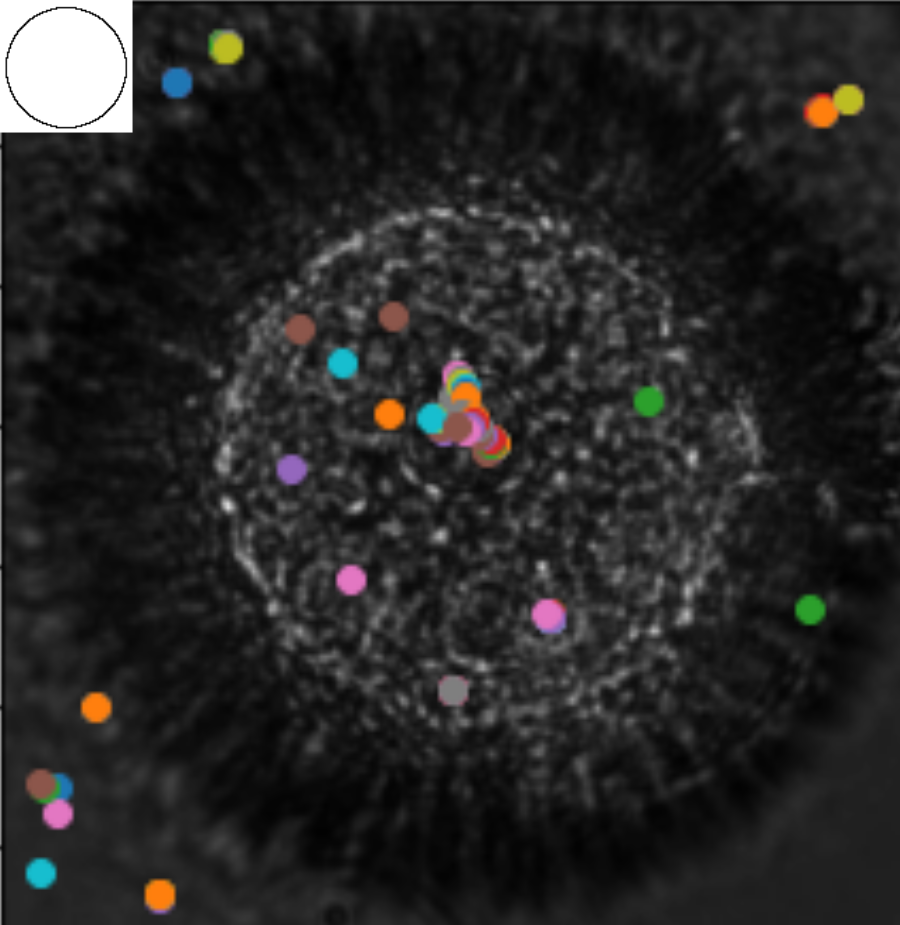
\includegraphics{mask-and-result}
  \caption{The mask used for corrTrack in the upper left corner.
  The result of the tracking is shown as colored circles, where different colors denote different times.}
  \label{fig:mask-and-result}
\end{figure}

The preliminary result of the tracking is shown in Fig.~\ref{fig:mask-and-result}.
While in some frames the software locates the inner droplet correctly, in most frames, however, the detection is erroneous.
Overall, the tracking does not work well.
To improve the quality of the tracking, we can
i)improve the image quality by adding fluorescent dyes to the inner droplets,
ii) use a specific mask, instead of a binarized mask and
iii) crop the image to avoid false tracking outside the droplets.

In a new set of images obtained with bright-field microscopy (Fig.~\ref{fig:bright-field-images}), I tested the ideas above.
As can be seen from the images, the inner droplets stand out from the background much better than the old images, so fluorescence is not necessary.
We tried 3 different masks:
i) an actual image of the inner droplet cropped from the first frame of the video,
ii) a black circle of the same shape as the inner droplet on a white background and
iii) a white circle of the same shape as the inner droplet on a black background (as shown in Fig.~\ref{fig:3-masks}).

\begin{figure}[h]
  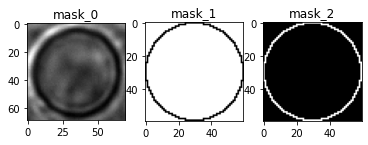
\includegraphics{3-masks.png}
  \caption{Three different masks.}
  \label{fig:3-masks}
\end{figure}

The raw image is also cropped to avoid false detection outside the outer droplet.
The results of corrTrack is shown in Fig.~\ref{fig:3-mask-results}.
The 3 panels show the results obtained using 3 different masks in Fig.~\ref{fig:3-masks} (same order).
The 3 red circles in each panel indicates the positions in the image that have the highest correlations with the masks.
None of the 9 circles detect the inner droplet position correctly.
\textbf{I conclude that corrTrack is not an ideal method for tracking the inner droplets in the X-Y plane.}

\begin{figure}[h]
  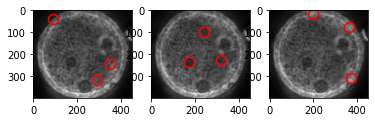
\includegraphics{3-mask-results.png}
  \caption{Tracking results using the 3 masks in Fig.~\ref{fig:3-masks}.}
  \label{fig:3-mask-results}
\end{figure}

\subsection{HoughCircles}

Due to the circular shape, the HoughCircles algorithm may be a good method for tracking the inner droplets.
Actually, I have used this method to measure the outer and inner droplet sizes, as described in the \textit{Drop size control} note.
The HoughCircles algorithm detects circular objects in images based on pixel intensity gradient.
While it can reliably detect the inner droplets, it also very often gives false positives, as shown in Fig.~\ref{fig:HoughCircles_false}.

\begin{figure}[h]
  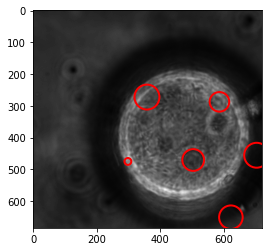
\includegraphics{HoughCircles_false.png}
  \caption{Results of HoughCircles algorithm.}
  \label{fig:HoughCircles_false}
\end{figure}

To overcome this challenge, I crop the original image so that the inner droplet makes the majority of the cropped image.
Using HoughCircles in the cropped image can avoid many false positives that are present in the original image.
By setting the minDist (the minimal distance between detected circles) large, e.g. the size of the cropped image, I can guarantee that at most one circle is detected (Fig.~\ref{fig:crop}).

\begin{figure}
  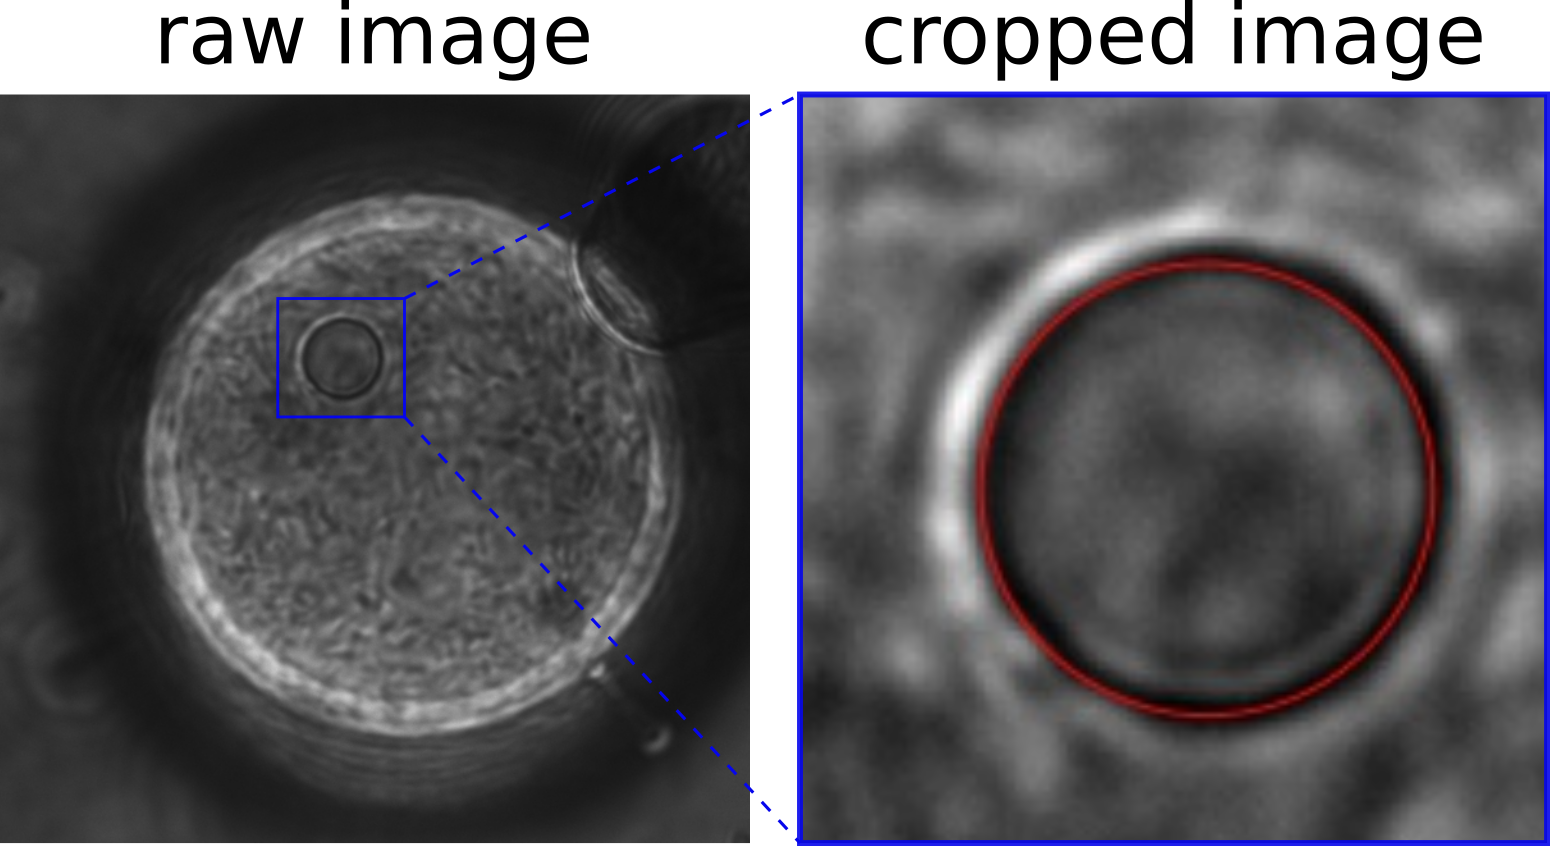
\includegraphics{crop.png}
  \caption{Detect circle in a cropped image.}
  \label{fig:crop}
\end{figure}

To implement the crop \& HoughCircles method on image sequences, an automatic way to determine crop regions is needed.
Here, as the first and simplest implementation, I assume the displacement of inner droplet between two frames (0.03 s) is negligible.
The position of droplet detected in the first image is used as the position of the crop region in the second frame.
This process can repeat to the end of the image sequence.
\textcolor{red}{In the next version, the crop regions will be predicted base on the instantaneous velocity of the inner droplet.}

\textbf{Exclude incorrect detections.}
Despite the effort of cropping, the HoughCircles algorithm sometimes makes mistakes.
Figure~\ref{fig:crop-HoughCircles-montage} shows a time series of cropped images in a crop-HoughCircles tracking.
The red circles indicate the results of tracking.
There are clearly two periods, where the tracking is incorrect: 400--740 and 1420--1760.
In other frames, the tracking is satisfactory.
I tried to restart the tracking in the middle of the image sequence and manually pick a crop region, but incorrect detection persists.
The problem is intrinsic to the algorithm rather than the crop region.
For now, I add a column ``validity'' to the trajectory data to indicate the validity of tracking at each frame: 1 for valid and 0 for invalid.

\begin{figure}
  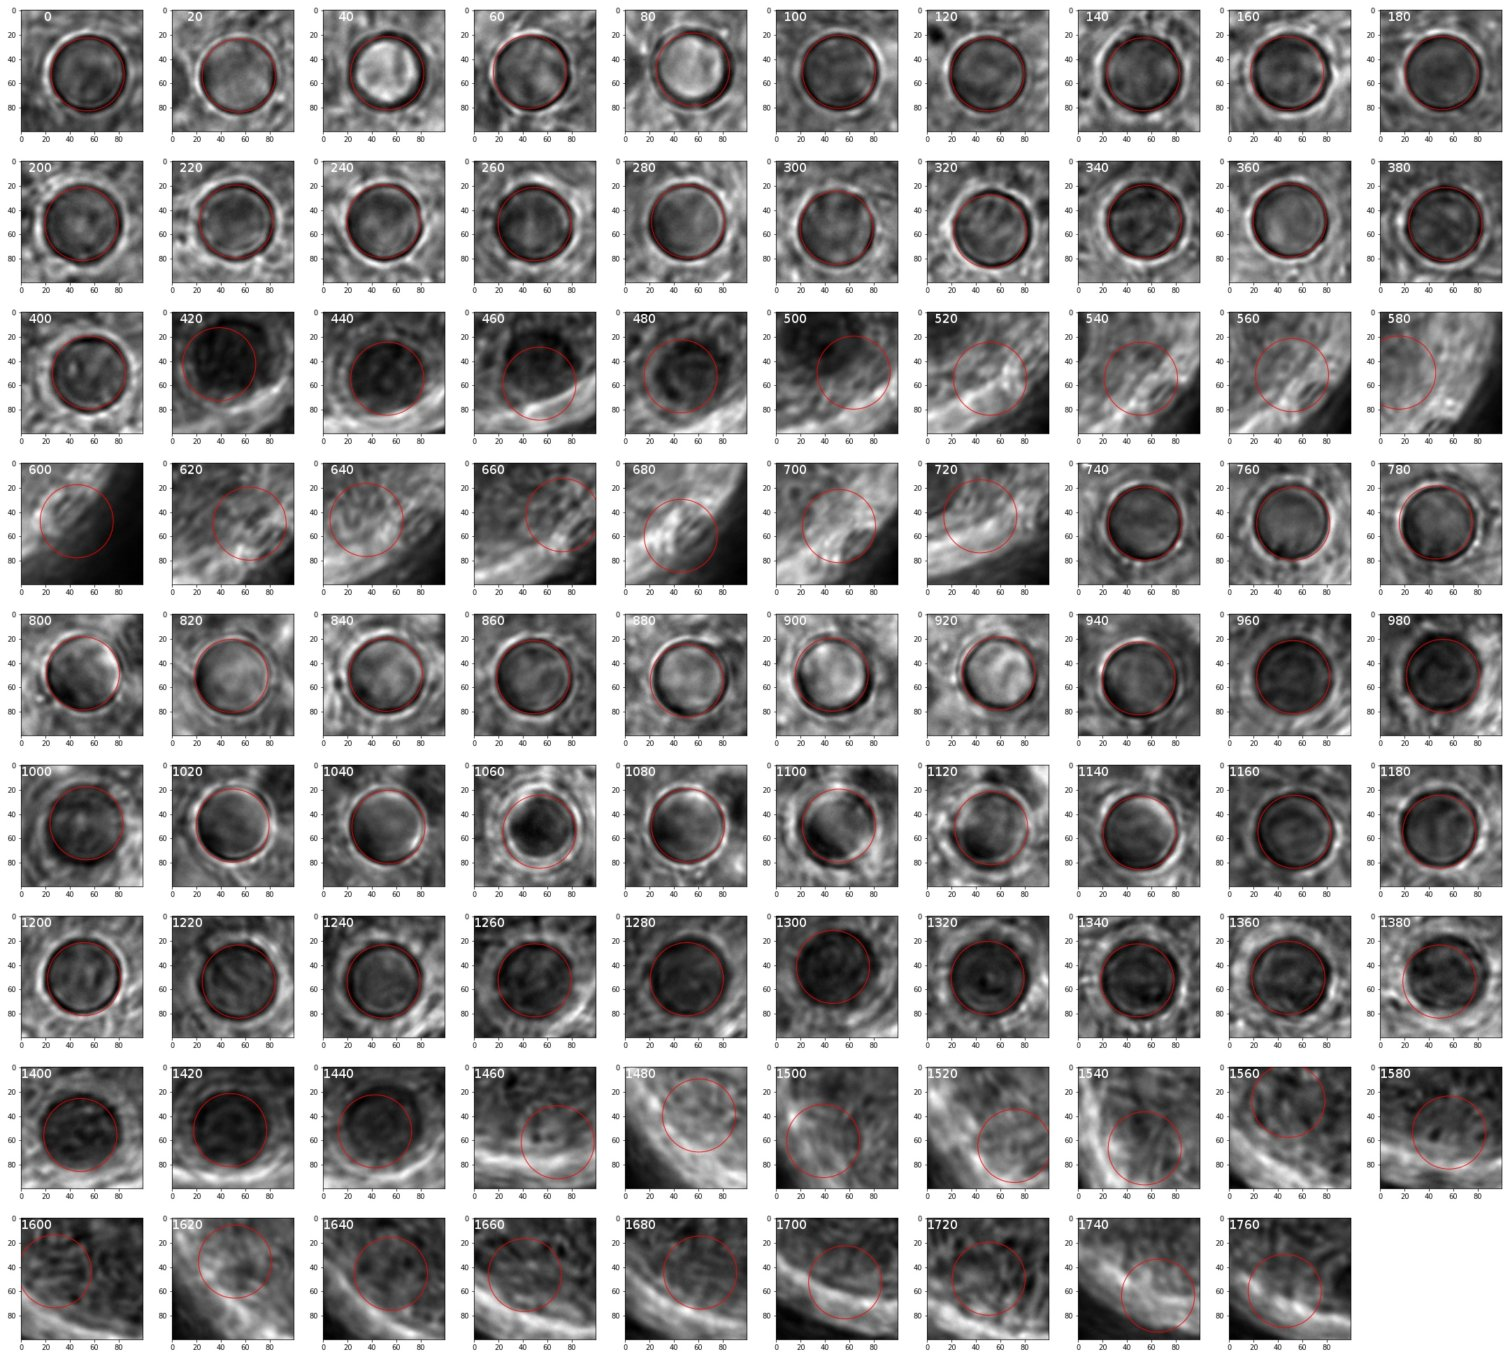
\includegraphics[width=6in]{crop-HoughCircles-montage.jpg}
  \caption{A time series of cropped images in a crop-HoughCircles tracking.}
  \label{fig:crop-HoughCircles-montage}
\end{figure}

\section{Z position}
As I wrote in the \textit{GOALS} note, the Z position of the inner droplet is crucial to understand the system.
On the one hand, we need the Z motions to interpret the dynamical properties, such as the diffusivity of the inner droplets we have measured in the X-Y plane;
on the other hand, it is a fingerprint behavior that should be compared with theoretical models.

We have proposed two ways to obtain Z positions: i) vertical scan and ii) tilted confocal.
Both methods have advantages and disadvantages.
Vertical scan can give X-Y position and Z position simultaneously.
But in each period of the scan, only one coordinate can be recorded.
Since the scan can not go as fast as the frame rate (typically 30 Hz), the resulting data would be sparce.
Confocal can record Z positions at a much higher rate, but simultaneously recording X-Y positions remains challenging.
\textcolor{red}{Test both options and assess.}

\subsection{Vertical scan}
The idea of vertical scan is illustrated in Fig.~\ref{fig:manual-scan}.
The inner droplet has slightly different lookings when it is in different positions relative to the focal plane.
When the droplet is below the focal plane, circular fringes can be seen around the droplets.
When the droplet is in the focal plane, the edge of the droplet is thin and sharp.
When the droplet is above the focal plane, the edge becomes thick and blurry.

\begin{figure}[h]
  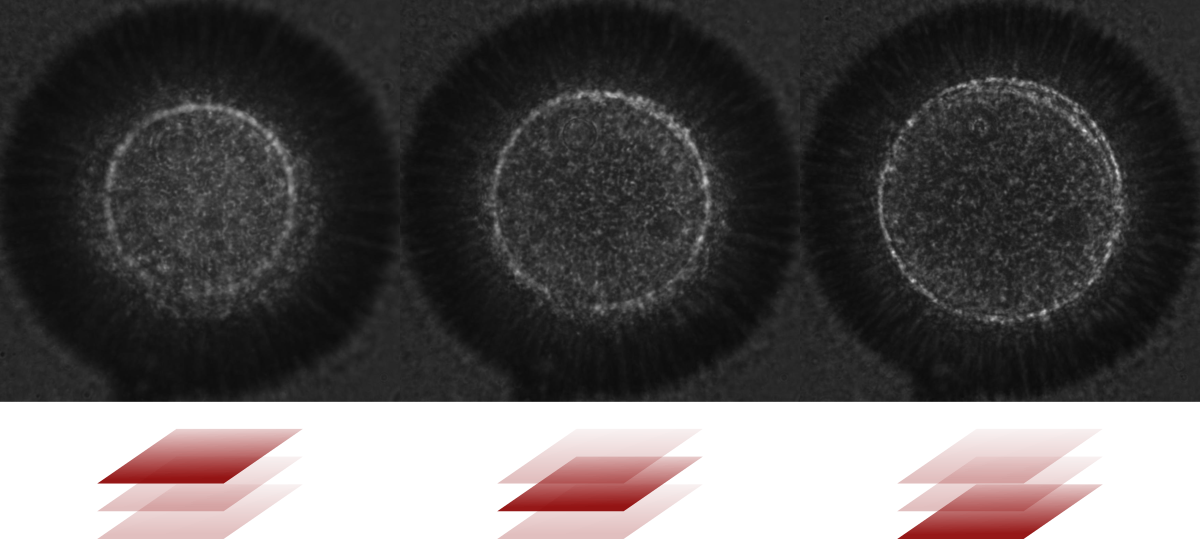
\includegraphics{manual-scan.png}
  \caption{Illustration of vertical scan of an O/W/O double emulsion. Images are from phase contrast microscopy.}
  \label{fig:manual-scan}
\end{figure}

Images in Fig.~\ref{fig:manual-scan} are from phase contrast microscopy.
The inner droplets can be seen, but the contrast with other parts of the images is weak.
This is troublesome when I try to track the droplets.
I imaged the same system using bright-field microscopy.
The images are shown in Fig.~\ref{fig:bright-field-images}.
Compared to the phase contrast images, the inner droplets stand out much more and should be easier to track.

\begin{figure}[h]
  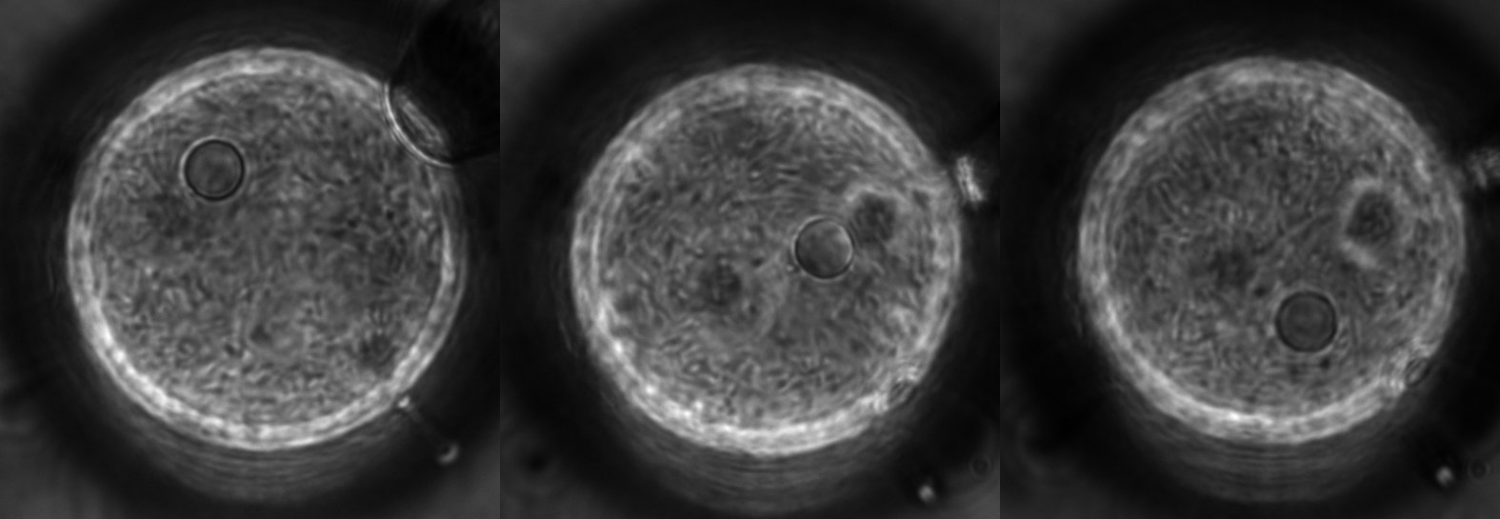
\includegraphics{bright-field-images.png}
  \caption{Bright-field images of an O/W/O double emulsion.}
  \label{fig:bright-field-images}
\end{figure}


\subsection{Tilted confocal}

\end{document}
